\fancychapter{Clustering Tweets with Self Organizing Maps}
\label{ch:clustering_tweets}

\section{Introduction}
\label{sec:adapting_the_som_to_the_social_web}

\section{Twitter Data}
\label{sec:crawling_twitter}
Twitter is a social network website and mobile app, where users are able to share whats on their mind with less than 140 characters. Due to its limitations, twitter users started to adopt their own kind of language on the social network, sharing shortened \ac{URL}, and tagging topics with a word preceded with an hashtag -- \# -- became so popular, that it was eventually implemented into twitter itself. Nowadays it is possible to monitor events through hashtags selections and links shared on the mobile app are automatically shortened.   

With the rise of smartphones and decent prices for mobile Internet access, and people becoming always online, GPS coordinates where also added to tweets. In fact a tweet nowadays has a massive amount of information, as can be seen in Figure~\ref{fig:json_tweet}.


There are two main ways to gather data from twitter: Crawl twitter HTML pages and scrap the intended information, access through the twitter API.

Crawling web pages is done through the analysis of HTML documents generated by twitter servers. Due to specific semantic rules, it is possible to gather almost all information that is possible to have access through the twitter API. Even though writing an HTML crawler is not particularly complex, specially through the usage of open source tools like nokogiri \footnote{http://www.nokogiri.org/} or beautiful soup \footnote{http://www.crummy.com/software/BeautifulSoup/}, Twitter specifically asks to not be crawled in some parts of their \ac{URL}, as can be seen in Figure~\ref{fig:twitterrobots}. 

Basically the restrictions that twitter asks on his robots.txt, only allows for search results, and hashtag searches to be monitored, which is pretty limiting.

\begin{figure}[htpb]
  \centering
  \begin{boxedverbatim}
  # Every bot that might possibly read and respect this file.
  User-agent: *
  Allow: /?lang=
  Allow: /hashtag/*?src=
  Allow: /search?q=%23
  Disallow: /search/realtime
  Disallow: /search/users
  Disallow: /search/*/grid

  Disallow: /*?
  Disallow: /*/followers
  Disallow: /*/following

  Disallow: /account/not_my_account

  Disallow: /oauth
  Disallow: /1/oauth
  \end{boxedverbatim}
  \caption{Twitter robots.txt piece where it is possible to see what should and shouldn't be crawled}
  \label{fig:twitterrobots}
\end{figure}

When accessing twitter through their API, authentication is required as since version 1.1. The authentication mechanism at hand, is used to limit the amount of information users can gather from twitter. 
The API itself is divided in the streaming -- used for subscribing directly to twitter public, user or site streams --  and REST -- used for programmatic access to read and write to the twitter API.  

The streaming API is extremely useful for building dataset based on keywords ,searches and entities. Since their API limit is based on levels, and the default level lets an endpoint track up to 400 words, and 5000 user ids as long as the amount of tweets streamed to the endpoint doesn't  surpass the 1\% of the total amount of tweets Twitter is currently streaming. Although, if some wrong terms are monitored, the amount of spam crawled can be huge, specially when monitoring public entities or trending hashtags. 

The REST API can be used to get all information that is available on twitter by the time the request is sent. REST API limits are much greater than the ones applied at the streaming API. The basic rules are 15 minutes windows per endpoint where 15 requests can be made. There are some exceptions to these rules and those can be found on twitter documentation \footnote{https://dev.twitter.com/rest/public}

\begin{figure}
  \begin{center}
    \begin{lstlisting}[language=json,firstnumber=1]
{ 
  "_id" : { "$oid" : "4fa14bc97e5617025fb14787" },
  "text" : "RT @FastCoDesign: A Paintbrush That Works On The iPad http://t.co/eWjEZAga (@sensubrushman)",
  "id_str" : "197701817864421376", 
  "coordinates" : null, 
  "in_reply_to_screen_name" : null, 
  "in_reply_to_user_id" : null,
  "possibly_sensitive" : false, 
  "favorited" : false, 
  "in_reply_to_status_id" : null, 
  "source" : "<a href=\"http://www.flipboard.com\" rel=\"nofollow\">Flipboard</a>", 
  "possibly_sensitive_editable" : true, 
  "contributors" : null, 
  "retweet_count" : 0, 
  "truncated" : false,
  "in_reply_to_status_id_str" : null,
  "geo" : null,
  "in_reply_to_user_id_str" : null,
  "entities" : { Enteties Object },
  "user" : { User object },
  "retweeted" : false,
  "id" : 197701817864421376,
  "place" : null,
  "created_at" : "Wed May 02 14:59:21 +0000 2012" }

    \end{lstlisting}
  \end{center}
  \caption{\ac{JSON} representation of a Tweet.}
  \label{fig:json_tweet}
\end{figure}



Due to the amount of specificity allowed by the REST API, it is better suited to create datasets that mimic the way twitter data is interconnected, like getting users and their followers, as well as their tweets.

\subsection{Crawling Twitter for Social Relations}
\label{sub:crawling_twitter_for_social_relations}
When trying to find clusters of topics with \ac{SOM}, integrating the social network in the output space the need for a dataset which had the social connections between the authors of the tweets arose.

Given the fact that the social relations where required, we opted for making a crawler based on the REST API. Due to the fact that twitter API rate limits would be achieved with some ease, the crawler should be prepared to achieve this maximum amount of requests per 15 minute window and wait for fifteen minutes. 

Also, at a given time, the crawler should be able to serialize it state in order to able to resume crawling in case its has to stop at any given worldly circumstances. 

\section{SOM}

\subsection{Clustering Tweets}
\label{sub:clustering_tweets}

In order to use \ac{SOM} to cluster tweets, first the tweets need to be converted into \ac{VSM}. Given the fact that tweets are often misspelled, with slang words and are written in multiple languages the \ac{VSM} tends to become pretty large with relative ease. 

The in order to reduce the amount of different words that could have the same meaning, or no meaning at all the following rules where applied:

\begin{itemize}
  \item Only English tweets where used during clustering.
  \item \ac{URL} are removed. Since most of them are minimized little information can be taken from them without domain translations.
  \item Numbers are removed.
  \item All letters are down cased.
  \item Runs of a character are replaced by a single character.
  \item Words smaller than 3 chars are discarded.
  \item Stop words are removed. 
  \item The tweet text is stemmed.
\end{itemize}

By applying these rules the \ac{VSM} is greatly reduced without destroying major relevant words. More information about \ac{VSM} reduction can be found on chapter X.

Since tweets are very small and have an average of only 10~14 words, there is no need to store term frequency on the \ac{VSM}, only a binary count is made.

Converting tweets from text to \ac{VSM} can be done in two different approaches: cumulative approach, where the \ac{VSM} is being built at the same time that the tweets are read, and as soon as a new term is found, it is a new position is added to the \ac{VSM} matrix. The second way relies on scanning all words present in the dataset in order to first build the \ac{VSM}, then iterate through all tweets and mark them as ones and zero's if they occur in the tweet text. 

After the \ac{VSM} is filled with tweets, it can be feed to the \ac{SOM} and training can start. It is important to notice though that since a destructive process was done to minimize the size of the \ac{VSM} if we want to read the tweets associated to clusters after the \ac{SOM} training, some extra mechanisms must be implemented.
{\color{red} write about the NLP and how it fits in all of these }
\subsection{Extensible SOM Library}
\label{sub:extensible_som_library}

When researching ways to extend the \ac{SOM} algorithm, in order to add social features to the learning process. I found that the number of \ac{SOM} libraries was not very extense. Even though, programing languages often used in \ac{ML} and Data Mining, such as Python or C++, have their how implementation of the \ac{SOM} algorithm. I've found that most of these libraries are made in such a way to be extremely fast, in order to take as much advantage from the hardware they are running on as possible. They often lack the modularity needed to adapt the \ac{SOM} algorithm to specific problems.

The \ac{SOM} algorithm has been changed many times in order to better categorize data with specific features, for example Geo-\ac{SOM} was described in Subsection~\ref{sub:types_of_soms}, the Growing Hierarchical \ac{SOM}~\cite[]{1058070}, the time adaptive \ac{SOM}~\cite[]{1187438}, the Ontological \ac{SOM}~\cite[]{5446427}, and the list goes on\dots  

In order to create the homophilic \ac{SOM}, described in Section~\ref{sec:algorithm_changes} we first created a \ac{SOM} framework that is easy to extend due to be fully object oriented, scripted --- even though it can be compiled to run on the JVM --- and without C extensions.



\section{Homophilic SOM Definition}
\label{sec:algorithm_changes}
The default \ac{SOM} algorithm has no idea whatsoever of the social connections between the tweets, it simply looks at the binary vectors that represent sentences and assigns it to the most similar neuron.

In order to better categorize socially connected data, we propose some alterations to the \ac{SOM} algorithm in order to make it aware of the social connections between the tweets, and therefor better represent the homophilic behavior present on social networks.

\subsection{Output Space}
\label{sub:output_space}
The outputs space is the zone on the \ac{SOM} algorithm where the neurons reside. It works like a cortex where neurons are scattered in a geometric fashion, generally a square. The output space is generally initialized with random values, with a relatively high learning rate, and also a relatively high number of epochs. The algorithm is made this way in order to be able to identify any type of data that can be represented as vectors.

First we will try to change the output space to better resemblance the social network. In order to do this, the squared grid that defines the output space was changed by the social network connections, and the neurons, are represented by a social network user. This changes are applied in the following way:
\begin{figure}[htpb]
  \centering
  \subfigure[The neighbourhood is defined by the relations of followers/followees between the winning neuron and the other neurons]{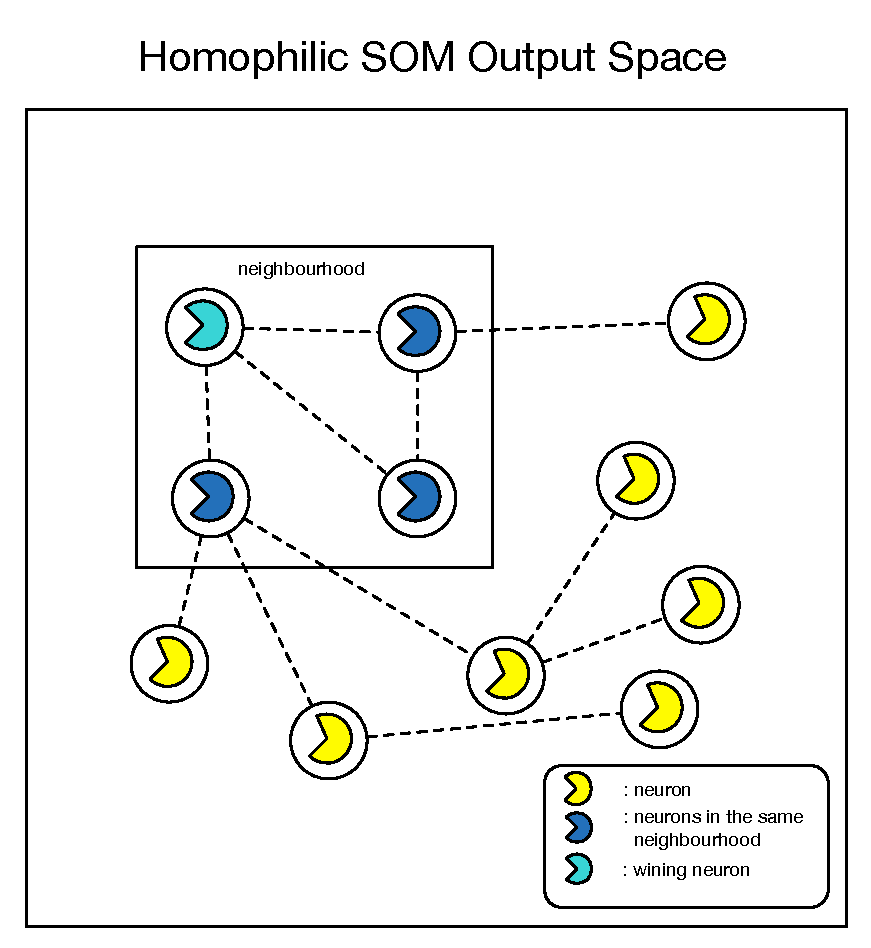
\includegraphics[scale=0.3]{./images/homophilic_outputspace.pdf}\label{chp3:homout}}
  \hspace*{0.5cm}
  \subfigure[Homophilic input space works in the same way as a normal input space]{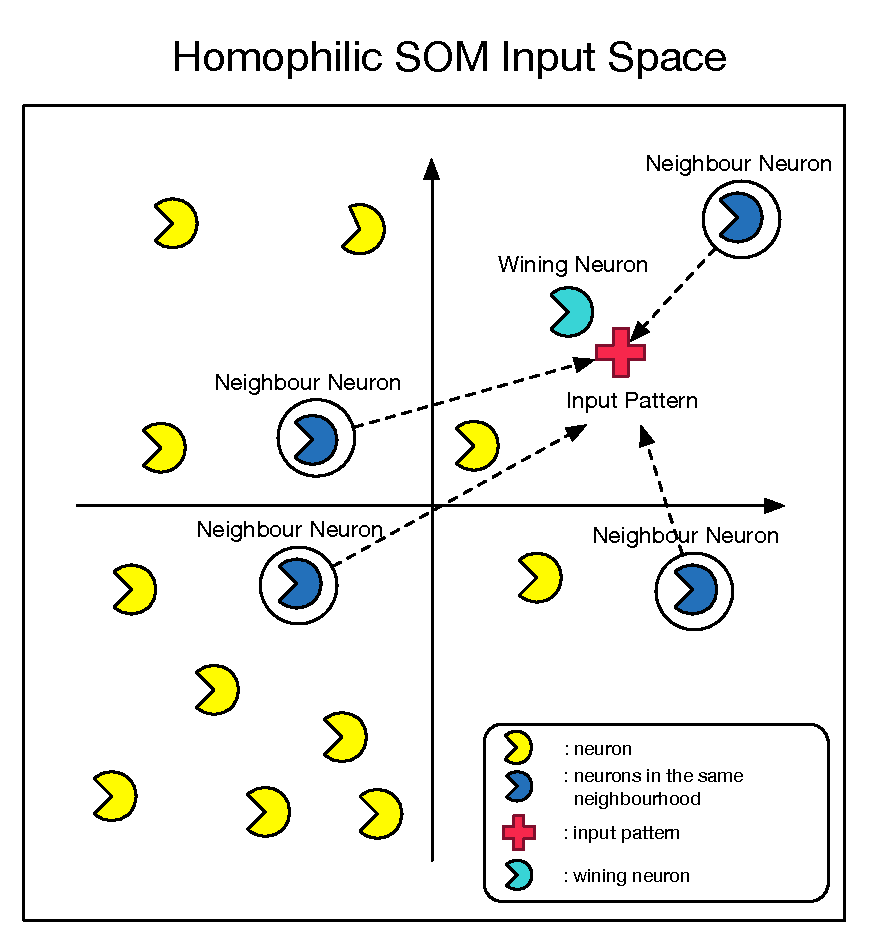
\includegraphics[scale=0.3]{./images/homophilic_input_space.pdf}\label{chp3:homin}}
  \label{fig:homo_in_out}
  \caption{ Homophilic SOM output and input space during the learning phase. }
\end{figure}
\begin{itemize}
  \item Each neuron is comprised of the text from all the tweets that he authored.
  \item Each neuron has a unique id, and stores the ids of his followers and followees that are present in the output space.
  \item During the learning phase, the radius will be defined as the maximum number of hops separating the winning neuron and followers/followees of followers/followees. 
  %\item Each neuron will cache followers/followees of a follower/followee to a specified depth level, for performance purposes. 
\end{itemize}


\subsection{Learning Phase}
\label{sub:learning_phase}
Like in the default \ac{SOM} the learning phase is where the output space is trained in order to organize the input data into clusters. Since this algorithm is specific to categorize tweets using social network features, the learning rate, radius and number of epochs used can be greatly reduced in order for the algorithm to converge. The learning phase operates in the following way:

\begin{itemize}
  \item The distance between the input pattern and all the neurons is calculated. The neuron closest to the input pattern is considered the winning neuron.
  \item When the winning neuron is selected, he and his social neighbors within k hops, update their representations in the input space, and move closer to the input patter. The Gaussian function (Func.~\ref{eq:gaussian}) is also used in here in order for the neighbors that are closer to the input pattern be significantly more influenced by the input pattern, while the neurons further away are less influenced. 
  \item This process is repeated for a predefined number of epochs. While the number of epochs increases, the learning rate, and number of hops that defines the neighborhood decreases in order for the algorithm to converge.
\end{itemize}

Just like the default \ac{SOM} algorithm, after the map is trained, input patterns can be fast assign to the nearest neuron since the neuron positions in the output space are no longer updated.

\subsection{Visualizing Neuron Representation Quality}
\label{sub:visualizing_neuron_representation_quality}
The homophilic \ac{SOM} has an output space that doesn't relate to any kind of geometric figure, due to this fact it is not possible to visualize the clusters formed using \ac{U-Matrix}. In order to solve this problem we propose an alternative way to visualize \ac{SOM} that instead of focusing on the distance between the neurons on the output space -- like the \ac{U-Matrix} -- it focuses on the mean quantization error between each neuron and the input patterns it is mapped to. We named this method Q-Matrix ( All. \ref{alg:qmatrix} ) due to its similarity to the \ac{U-Matrix} but using the mean quantization error.

\begin{figure}[h]
  \begin{algorithm}[H]
    \label{alg:umatrix}
    \DontPrintSemicolon
    \KwData{Input patterns $X = \{  \overrightarrow{x_1}$,\dots,$\overrightarrow{x_N}$ \}, Trainned neurons $W = \{  \overrightarrow{w_1}$,\dots,$\overrightarrow{w_N}$ \} }
    \KwResult{U-Matrix}
    \For{ $w_d = \overrightarrow{w_1}$ to $\overrightarrow{w_N}$ }{
      (NOTA: Nao sei muito bem como escrever isto numa formula matematica..) the average of all the distances between a neuron and all of the input patterns he represents
      }
      \caption{U-Matrix }
  \end{algorithm}
\end{figure}


The algorithm works in the following way: for each neuron in the grid, we find the quantization error between it and all the input patterns it represents. Afterwards we calculate the average between all the quantization errors associated to the neuron, and add it to the Q-Matrix. After this process is applied to all neurons, all quantizations errors are converted to a color that is directly proportional to the amount of the mean quantization error. 

Even though we used the Q-Matrix algorithm to find the best clusters on the Homophilic \ac{SOM} where each neuron represents a cluster. The Q-Matrix can be applied to the default \ac{SOM} algorithm in order to easily visualize neurons which don't represent well their input patterns. An example of a Q-Matrix can be seen in Figure~\ref{fig:som_trqmatrix}
\begin{figure}[htpb]
  \centering
  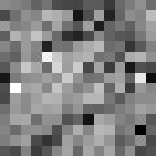
\includegraphics[scale=2]{./images/som_training/2_quantmatrix.pdf}
  \caption{Q-Matrix calculated after 300 epochs of training a default \ac{SOM} algorithm to identify colors. By looking at the matrix it is very easy to see which neurons are not representing their associated input patterns well -- in black -- and in white the ones that have very little quantization error and therefor are good at representing their input patterns}
  \label{fig:som_trqmatrix}
\end{figure}

